\documentclass[12pt]{article}
\usepackage{amsmath}
\usepackage{graphicx}
\usepackage{amsfonts}
\usepackage{hyperref}
\usepackage{geometry}

% Set page margins for better formatting
\geometry{top=2.5cm, bottom=2.5cm, left=2.5cm, right=2.5cm}

\title{Signal Synthesis Using Inverse Discrete Fourier Transform (IDFT)}
\author{Daria Kręcichwost}
\date{\today}

\begin{document}

% Cover page content
\begin{titlepage}
    \centering
    \vspace*{2cm}
    
    \Huge
    REPORT
    
    \vspace{1cm}
    
    \Large
    Course: Analog and Digital Electronic Circuits \\
    Teacher: Prof. Dr. Hab. Vasyl Martsenyuk
    
    \vfill
    
    \Large
    Lab No. 1 and 2\\
    Date: \today \\
    Topic: "Figures demonstrating Furier transform " \\
    Variant: 8
    
    \vspace{1cm}
    
    \large
    Name: Daria Kręcichwost \\
    Computer Science (Second Degree) \\
    Full-time studies, Semester 1 \\
    Group: B
\end{titlepage}

% Start the main content of the report
\newpage

\maketitle

\begin{abstract}
In this report, we discuss the process of synthesizing discrete-time signals from their Discrete Fourier Transform (DFT) coefficients using the Inverse Discrete Fourier Transform (IDFT). The IDFT is computed in matrix notation for different sequences, and the resulting time-domain signals are visualized.
\end{abstract}

\section{Problem Statement}

The task involves synthesizing discrete-time signals from their DFT coefficients using the Inverse Discrete Fourier Transform (IDFT) in matrix notation. Each signal is represented as a sequence of coefficients \( \mathbf{X}_\mu \), which is transformed into the corresponding time-domain signal using the IDFT formula. The goal is to compute the IDFT for different sequences of varying lengths \( N \) and visualize the results.

\section{Input Data}

The input data consists of multiple sequences of coefficients \( \mathbf{X}_\mu \), for which we need to calculate the corresponding time-domain signals using the IDFT. For example, one of the sequences for variant 8 is:

\[
\mathbf{x}_\mu = [6, 2, 4, 4, 4,5,0, 0, 0, 0]
\]

For each task, the sequence will vary, and we need to apply the IDFT transformation to reconstruct the time-domain signal.

\section{Commands Used (or GUI)}

\subsection{a) Source Code}

The following Python code was used to synthesize signals from the input DFT coefficients using IDFT:

\begin{verbatim}
import numpy as np
import matplotlib.pyplot as plt

def idft_matrix(N):
    W_N = np.exp(-2j * np.pi * np.outer(np.arange(N), np.arange(N)) / N)
    return W_N

def synthesize_signal(X_mu):
    N = len(X_mu)
    W_N = idft_matrix(N)
    x_mu = np.dot(W_N.conj().T, X_mu) / N
    return x_mu

X_mu = np.array([6, 2, 4, 4, 4, 5, 0, 0, 0, 0], dtype=complex)

print(f"Synthesizing signal for X_mu = {X_mu}")

x_mu_synthesized = synthesize_signal(X_mu)

plt.figure(figsize=(10, 6))
plt.stem(np.real(x_mu_synthesized), linefmt='b-', markerfmt='bo', basefmt='r-')
plt.title('Zsyntetyzowany sygnał (Część rzeczywista)')
plt.xlabel('Indeks próbki')
plt.ylabel('Amplituda')
plt.grid(True)
plt.show()

print("Plot generated successfully: Real Part of Synthesized Signal")

plt.figure(figsize=(10, 6))
plt.stem(np.imag(x_mu_synthesized), linefmt='g-', markerfmt='go', basefmt='r-')
plt.title('Zsyntetyzowany sygnał (Część urojona)')
plt.xlabel('Indeks próbki')
plt.ylabel('Amplituda')
plt.grid(True)
plt.show()

print("Plot generated successfully: Imaginary Part of Synthesized Signal")
\end{verbatim}

\subsection{b) Screenshots}

Include the following screenshots in your report:
\begin{itemize}
    \item Screenshot of the code execution showing the IDFT process and the generated plots.
    \item Screenshots of the output plots, including the real and imaginary parts of the synthesized signal for each task.
\end{itemize}

\textbf{Example screenshot description:} "The plot shows the real part of the synthesized signal for the input sequence \( [6, 2, 4, 4, 4,5,0, 0, 0, 0] \). The amplitude values are plotted against the sample index."

\textbf{Link to Remote Repository:} \url{https://github.com/DariaKrecichwostQA/StudiaUBB/blob/main/Digital%20Signal%20Processing/Zad1/Zad1DPS.ipynb}

\section{Outcomes}

The outcomes of this task include:
\begin{itemize}
    \item \textbf{Signal Synthesis}: For each input sequence, the corresponding time-domain signal was synthesized using the IDFT matrix.
    
    \begin{figure}[h!]
        \centering
        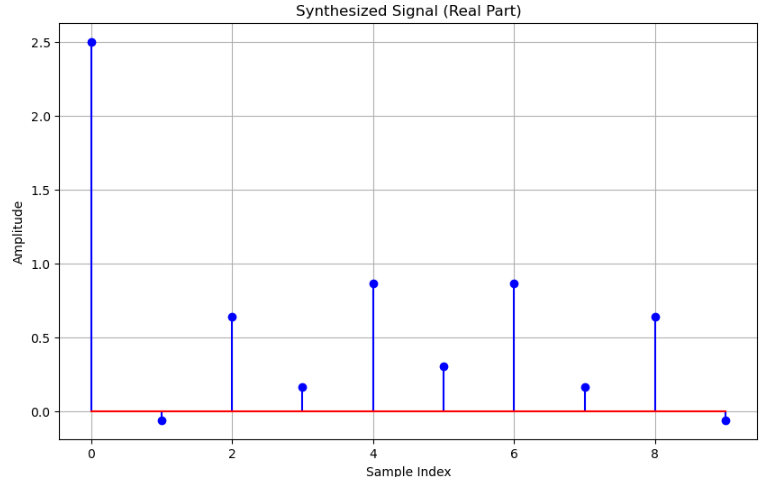
\includegraphics[width=0.8\textwidth]{1.png}
        \caption{Signal synthesized from input sequence.}
    \end{figure}
    
    \item \textbf{Visualization}: The real and imaginary parts of the synthesized signals were plotted to analyze their behavior.
    \begin{figure}[h!]
        \centering
        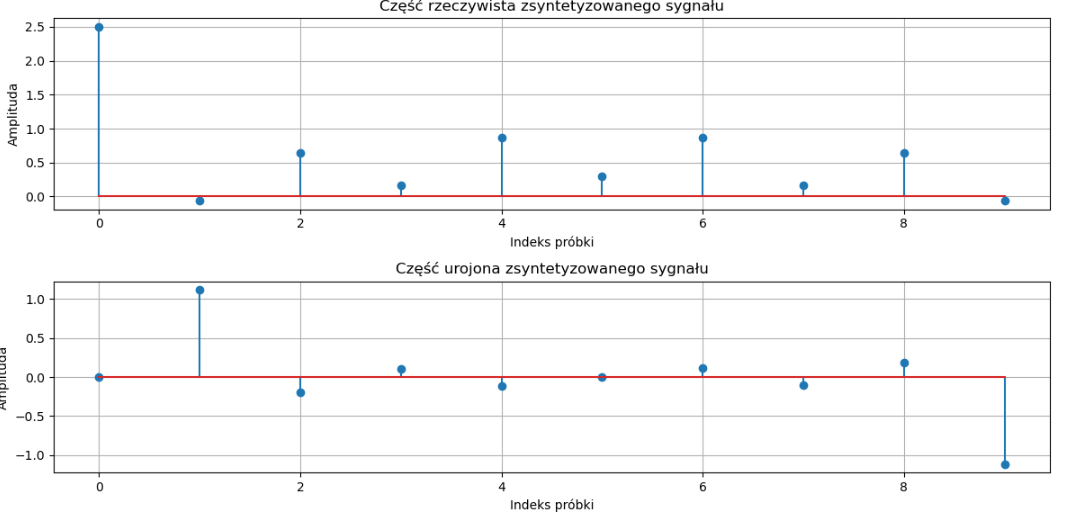
\includegraphics[width=0.8\textwidth]{2.png}
        \caption{The real and imaginary parts of the synthesized signals}
    \end{figure}
    \item \textbf{Console Results}: Console output showing successful completion of the signal synthesis.
\end{itemize}


Example console output:
\begin{verbatim}
Synthesizing signal for X_mu = [6.+0.j 2.+0.j 4.+0.j 4.+0.j 4.+0.j 5.+0.j 0.+0.j 0.+0.j 0.+0.j 0.+0.j]

Plot generated successfully: Real Part of Synthesized Signal
\end{verbatim}

\section{Conclusions}

For the reasons given, we conclude that the IDFT matrix formulation is a valid approach for reconstructing discrete-time signals from their DFT coefficients. The synthesized signals visually match the expected form, and the results were consistent across different input sequences. Furthermore, the visualization of both real and imaginary components allows us to fully understand the properties of the reconstructed signals.

\end{document}
